\documentclass[conference]{IEEEtran}
\usepackage{cite}
\usepackage{tcucosc}
\usepackage{lipsum}


\title{Parallelized Traffic Simulation in C++}

\author{
\IEEEauthorblockN{Zach Alaniz}
\IEEEauthorblockA{Department of Computer Science\\
College of Science and Engineering\\
Texas Christian University\\
Fort Worth, Texas 76129\\
Email: z.a.alaniz@tcu.edu\\}
\and
\IEEEauthorblockN{Saby Sahoo}
\IEEEauthorblockA{Department of Computer Science\\
College of Science and Engineering\\
Texas Christian University\\
Fort Worth, Texas 76129\\
Email: s.sahoo@tcu.edu\\}
\and
\IEEEauthorblockN{Bradley Schoeneweis}
\IEEEauthorblockA{Department of Computer Science\\
College of Science and Engineering\\
Texas Christian University\\
Fort Worth, Texas 76129\\
Email: b.schoeneweis@tcu.edu\\}
}



\begin{document}


\maketitle


\begin{abstract}
This semester research project investigates the potential speedups and scalability of running a traffic simulation in parallel using C++ and OpenMP. These speedups are evaluated by comparing the sequential performance to the parallel performance when varying thread counts for a fixed-size, randomized input. While a large percentage of the program is inherently sequential due to computation, the process of transitioning from one state to another was parallelized. 
\end{abstract}
\bigskip
\begin{IEEEkeywords}
OpenMP, Cellular Automata, Parallel Simulation, C++
\end{IEEEkeywords}

\section{Introduction}
Extensive research and improvements have been made over the years in the field of study that is parallel computing. Falling within this domain of study is the topic of distributed simulation. As models become more and more complex, the execution time associated with these simulations becomes far too substantial for a sequential approach. A common remedy to this issue is to redesign the simulation to run in parallel. This research aims to see the benefits of running a parallelized discrete event simulation, and more specifically, a parallelized traffic simulation, over a sequential simulation. \cite{Fujimoto:1990:PDE:84537.84545} \\

The ability to optimize light scheduling and move cars from one point to another in an efficient, organized manner is paramount for day-to-day travel. Being able to apply parallel computing to simulate increasingly large traffic environments leads to many interesting research topics and advances in road safety, traffic capacity, economic impact, among many others. The topic of simulating traffic flow for increasingly large sizes of roads is the topic of interest explored in this simulation. Real life traffic flow allows for movement when possible at all times, and by utilizing parallel computing paradigms and tools, the speedup of a traffic simulation should prove beneficial in seeing how a particular road and intersection scales for an increasingly large number of cars funneling in and out.  \\

Traffic simulation naturally lends itself to parallel computing paradigms. Decomposing the movement of cars into a sub-domain of problems and updating traffic flow in parallel from one state to another, just as normal traffic would run, is one method to improved performance. 
Thus, a parallel solution to traffic flow needs to be able to parallelize any movement and update that could be happening concurrently. The dynamic nature of traffic also plays a large role in this type of simulation but was handled to leave a larger emphasis on the updating of car movements. The following research being presented simulates traffic flow through a four-way stop, which includes two-lane roads from all directions. The traffic simulation was built with C++ utilizing a cellular automaton approach.  The parallelization was made with OpenMP, an application programming interface (API) that supports shared memory multiprocessing. \\

The following is an overview of the remainder of the paper: Background research on the applied tools and ideas used and reasons for why they were chosen, the sequential algorithm design and solution, the parallelization and results, and finally a summary with conclusions of the research.
 \\


\section{Background and Related Research}
Chances are if you have ridden in a vehicle, you have come across a four-way stop being controlled by traffic lights. A four-way traffic stop has roads leading from all four directions (North, South, East, West) where each direction takes a turn moving towards its destination as directed by the controlling traffic light. The traffic light operates in three states: red, green, and yellow. Green means go, red means stop, and yellow means slow down. Assuming each direction is at least a two-lane road, and ignoring the possibility for a one-way street, any car driving on the outer most lane is capable of taking a right turn at the traffic light intersection if oncoming traffic is clear, regardless of the state of the light. Cars in the innermost lanes are also capable of making a left turn, given that their light is currently green. The light itself cycles on a timer allowing for each lane to have its own turn to proceed, which creates the flow of traffic. This four-way model is what our simulation is derived from, which will be explained in a later section. \\

The placement of cars along any road is relatable to a data model studied in computer science and related fields known as \textit{cellular automata}. Formally, cellular automata are defined as a collection of cells on a grid that evolves during a number of discrete time steps according to a set of rules based on the states of neighboring cells. The rules are then applied iteratively for as many time steps as desired \cite{WolframCellularAutomaton}. Cellular automata have been studied since the early 1950’s and was initially used as a model for biological systems. The lattice structure and discrete state like approach of cellular automata was taken and applied to our simulation to represent individual, discrete states of traffic flow and positions of cars within a street.  Another principle of cellular automatons is localized interactions with nearby cells.  Each car within this system must recognize the state of the cell that lies a step ahead in the direction it wishes to move in order to determine its next state. The different discrete representations of the states and interactions of the cars, the lights, traffic, and lanes in general will be explained later within the paper. \\

The general structure of the system has been described, now let’s look at the tools and technologies used to implement the simulation. The entirety of this research project was developed in C++ 17.  C++ is a statically-typed, compiled, middle-level, general purpose programming language developed by Bjarne Stroustrup in 1979.  C++ was used to implement all of the simulation logic and sequential transitions.  To parallelize this program, we used OpenMP. OpenMP is an Application Program Interface (API) that provides a portable and scalable shared memory model for parallel applications. OpenMP is designed for shared memory parallel programming. This was essential for our project.  What drove us to choose OpenMP over MPI (Message Passing Interface), which doesn’t have a concept of shared memory, was the potential costs of communication if the simulation were to be run with an input size of 200,000,000.  This would require an MPI implementation to have the processes broadcast the global automata system for every discrete state, which could be incredibly costly at scale.  With OpenMP, this global system can be shared memory and operated on by all the threads, without the overhead of frequent, massive scale communication instructions for all processes to get back on the same page. Another common parallelization library is POSIX threads (or pthreads). We chose OpenMP over pthreads due to critical section concerns and keeping the threads in sync while accessing the shared data simultaneously.  Pthreads offered too fine-grained control for the needed operations our system performs, and the flexibility given was overkill for this simulation's purpose.  OpenMP is more high level than pthreads, and allowed for easier, more accurate division of tasks among processes. As a result, OpenMP was the parallelization tool of choice for this project. \cite{openmp} \\

Now that the technologies and techniques have been selected to maximize our simulation specifications, a resource is needed for the execution, testing, and analysis of our program. In order to run high intensity simulations, for both thread count and input size, we would submit our project for execution as a batch job onto the Stampede2 computing cluster. Stampede2 is the flagship supercomputer at the Texas Advanced Computing Center, and consists of 1,736 nodes, and each has 48 cores and 192GB of RAM. This enabled us to run simulations with threads varying from one up to 64 threads on input sizes ranging from 200 to 200,000,000. \cite{stampede2}
 \\

With all resources in hand, we can discuss the history of traffic models. Parallelized traffic simulations have been implemented before and have evolved from relatively simple systems to very complex models.  Here are some of the implementations that inspired the following research, and set the path for modern, parallel traffic simulations. One of the very first cellular automaton-based simulations was designed by Nagel and Schreckenberg.  This simulation was developed for single lane traffic and was initially sequential.  It utilized Monte-Carlo methods to describe start-stop waves as traffic grows more and more dense.  While relatively simple, this model was used for traffic forecasts and analysis for years. As systems began to adapt multiple lanes of traffic and simulations were adapted to model high-density, urban areas, the need for parallelization quickly became realized. One of the first thoughts for parallelization was decomposing the automaton into sub-systems. The issue with this approach was something we also discovered from testing, was that the communication overhead when the system scales becomes far too costly for efficient execution.  Another approach that researchers sought out was dividing the system into preexisting time segments and eventually synchronizing the time slices. This also was not effective, as the outcomes of these time slices cannot be predetermined, as there must be an essence of randomicity to keep the simulation true.  Modern traffic parallelization utilizes methods for accurate systematic predictions to decompose the system into micro-states and optimize the computation to set-up the next state of the system while load-balancing the system splits to prevent massive communication costs. \cite{1443306} \\

Where this research project attempts to differentiate itself is by simplifying some of the logic of the random states and primarily focus on the parallelization of the state transition without decomposition. The hope is that at a large enough scale, our state transitions of even massive systems will be able to see performance improvements through OpenMP parallelization.  To do this, we have essentially simplified the next state logic for our four-lane simulation to adhere to a transition function of simply shifting each of the lanes towards the next determined state (computed prior to shift time).  The next section of this paper will discuss the sequential implementation of the traffic simulation, how the states are determined, and the operation to transition from one discrete state to another.
 \\

\section{Serialization Technique}

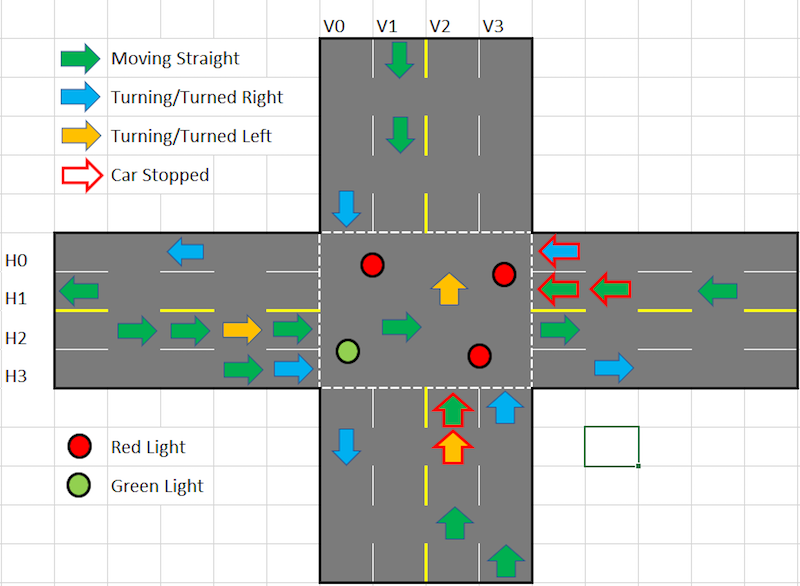
\includegraphics[width=0.45\textwidth]{images/traffic}
\begin{center}
	\textbf{Fig. 1} Overview of simulation  \\
\end{center}


To design our serial solution to the four-way traffic simulation, we began by deciding on using an array type data structure to represent each lane and store car states. Since our simulation runs with four horizontal lanes handling cars moving east and west, and four vertical lanes handling cars moving north and south, our solution uses eight arrays in total to hold all data. An array data structure was chosen for a few reasons. The first being because C++ arrays store memory contiguously, meaning the data is laid out next to each other with no gaps in between. This type of memory layout is ideal because it makes data parallelization simple, as well as allows for the use of the cellular automata model. Data layout was the reason that moved design away from an object-oriented approach. Storing objects in C++ leads to offsets between data in memory based on the data within each object, making it much harder to parallelize when the time comes. Within each of the eight arrays (roads) holds a variable number of cars throughout represented by an integer value of $0, 1, 2, $ or $3$. Each number corresponds to a specific action a car will be taking within the simulation. Each integer is defined as follows:\\ 

\begin{itemize}
	\item 0: Empty
	\item 1: Car moving straight
	\item 2: Car taking a right
	\item 3: Car taking a left \\
\end{itemize}

The eight roads included in the traffic simulation also result in a $4x4$ intersection point made of $16$ cells. This intersection point represents the cars that are moving to the other side of the road during a green light. To keep track of cars within this intersection point at any time, we split the work between horizontal and vertical, where either of the horizontal and vertical arrays can be holding cars within the intersection at any state. \\

Another important aspect to consider when designing the simulation was how to handle light timing for every road. To have our traffic lights continuously looping, a rotating array was used that shifted a single value based on a timer, which moved the state of one light on to the next. This way the light timing would continuously run until the simulations end.\\

\hspace*{.2cm} Two different approaches were used as input to populate our roads for simulation. The first was input by csv, where the csv was filled with numbers representing cars and could be read in to populate road data. 

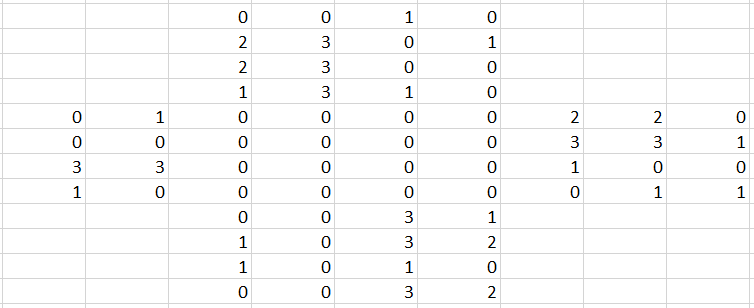
\includegraphics[width=0.45\textwidth]{images/input}
\begin{center}
	\textbf{Fig. 2} Example input file  \\
\end{center}

This input was useful when testing on smaller inputs and at the beginning of logic development, because it allows for controlled traffic states and expected output. The next type was randomized input. A command line argument is used to gather the dimensions of fo each road size and corresponding car types are randomly placed at every spot within each road based off of probability. This version of input allowed for increasingly large input sizes to be created and tested for more extensive testing once logic development was completed. It is also important to note that the beginning of any simulation cannot have cars starting within the intersection. So any type of input must leave the middle $4x4$ cells empty and allow cars to move up to the light at the start of simulating. \\

\hspace*{.2cm} To confirm correctness of development, an important output function was also created. The main version of output, which cleanly represents a traffic simulation, was done using UTF-8 characters to represent lights and prints to the console showing an overhead view of a current traffic state. \\

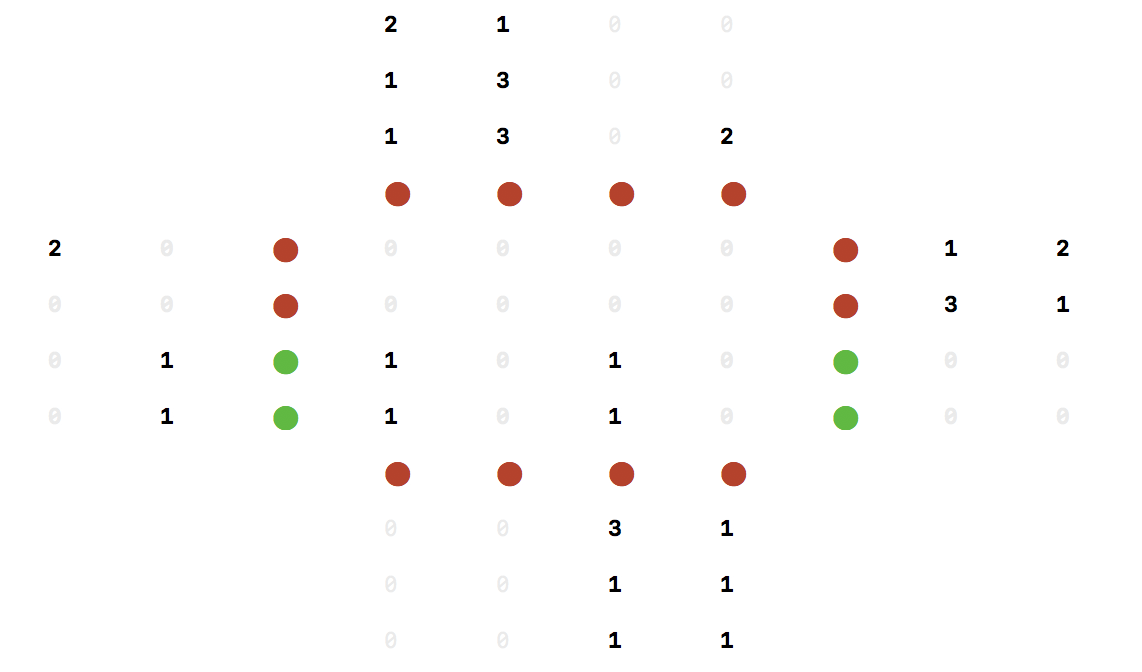
\includegraphics[width=0.45\textwidth]{images/output}
\begin{center}
	\textbf{Fig. 3} Example simulation output  \\
\end{center}


At any time, this output only represents the middle $20x20$ view of the traffic, including the $4x4$ intersection. This output leads to a minimum road size of 20 and allows for an easy view of the simulation regardless of the input size. So for an input size of $200,000$, the traffic can be visualized with many cars coming into and out of view. To go along with this, road statistics are also shown to know when the simulation will be ending, such as the number of car's exited, and how long each run of the simulation is takes. \\

\hspace*{.2cm} The updating of car positions is where cellular automata comes into the design. Each car is moved to its next state in the simulation by shifting them to the next spot in the array. This array shifting is done by indexing, which will prove to be of issue and explained later on. Before  a car can proceed, they must check ahead of them in the direction they are moving for an empty cell, which is in line with the model of cellular automata and checking states around one's current state. Throughout the simulation, cars are continuously checking states before moving through each cell until the simulation is complete. Updating the state of each road requires either a forward or backward loop depending on the direction the cars are moving. Cars moving to the east or south required looping from the end of the array, while those cars moving to the west or north required looping from the front. This is because updating the state of cars moving forward   requires the farthest most car to be updated before any car behind it, and the front most car is represented differently based on the direction of movement.\\

\hspace*{.2cm}  The simulation is run state by state until every car has exited. As the state simulation begins, each state is done one time followed by a short sleep time before the next state runs. To run the simulation, there is a pre-set sleep time that allows for state by state printing to the console between each step in the simulation. This sleep time can be lowered to run a faster simulation, and raised to run the simulation slower to analyze traffic. This set sleep time also controls the time each green light is set for, called light time, to scale it according to the speed and size of the simulation. Lastly, there is a clear time, which serves as the simulations yellow light, and allows for cars within the intersection to clear out before the next light becomes green. Green and yellow lights are calculated in the following way: \\

Light time $= sleep time \cdot factor$ \\

Clear time $= sleep time \cdot 4$ \\

where $factor$ is scaled to the size of the simulation. Clear time is always set to 4 because the intersection size is constant and any car would need at most 4 states to move out of the intersection point. \\

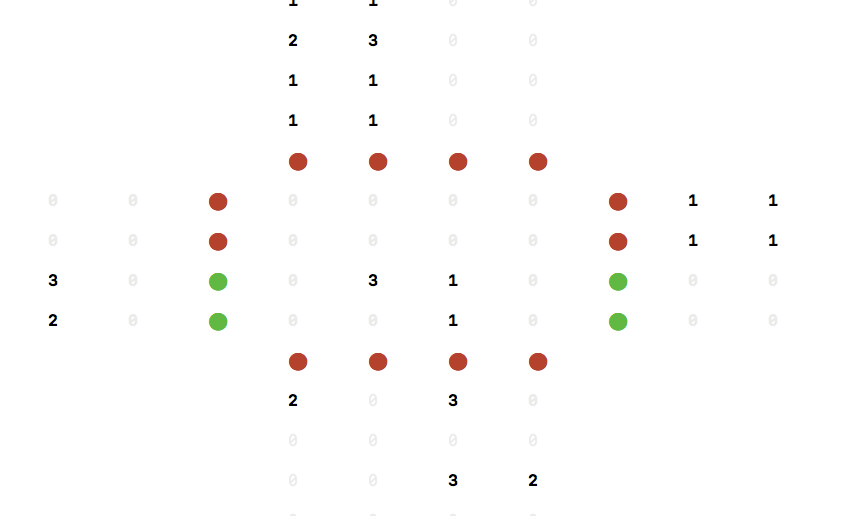
\includegraphics[width=0.45\textwidth]{images/green}
\begin{center}
	\textbf{Fig. 4} State during green light  \\
\end{center}

The above figure (Fig. 4) represents the simulation during a green light, where cars moving to the east are allowed to move forward. Cars in other lanes must wait unless they are turning red, which you see waiting behind each red light. \\

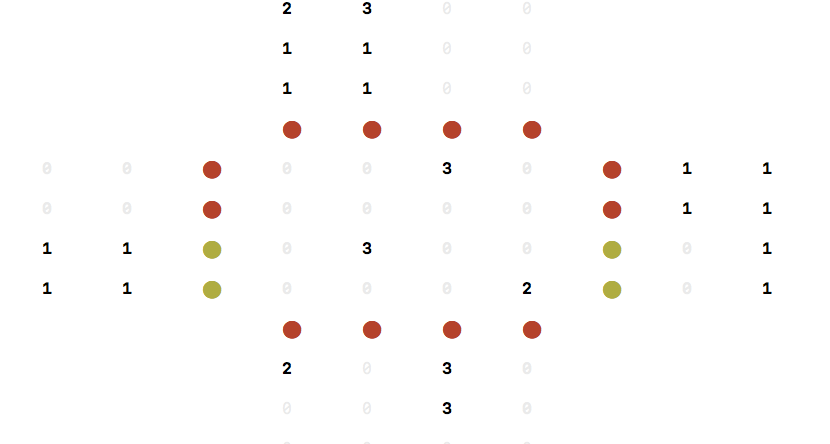
\includegraphics[width=0.45\textwidth]{images/yellow}
\begin{center}
	\textbf{Fig. 5} State during yellow light  \\
\end{center}

The next figure (Fig. 5) represents the simulation during a state of intersection clearing, or the yellow light state. During this time period, any cars within the intersection are moved forward to clear the road for the next light, which will be shown in the following image. \\

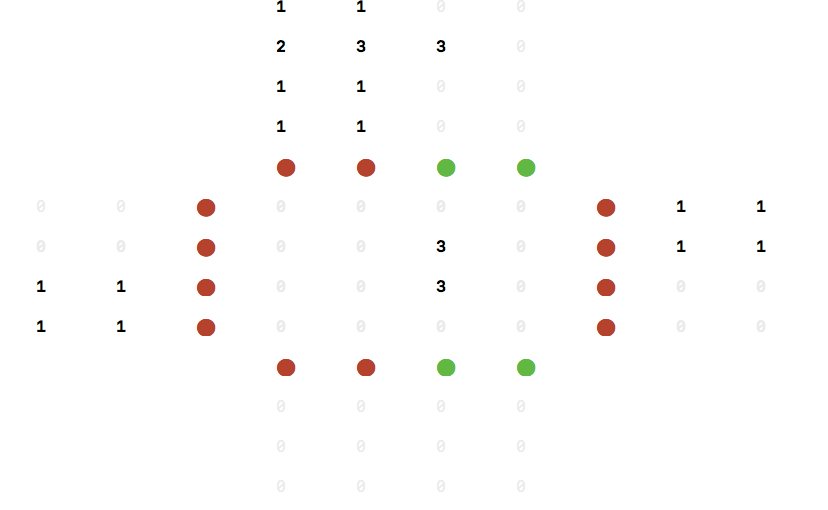
\includegraphics[width=0.45\textwidth]{images/red}
\begin{center}
	\textbf{Fig. 6} State during light change  \\
\end{center}

Once a yellow light is finished, the next light is set to green and those cars are allowed to move. Fig. 6 shows the next light turning green once the previous light states are finished. \\

\hspace*{.2cm} During green light states of the simulation, every car in the appropriate lane is moved forward in the direction the lane moves. Each movement is done by looping over the array and setting indices to be array[i] = array[i+1], or array[i] = array[i+1] depending on the direction. Any car that is labeled a 1 will not have to check for cars in front of them during a green light, since cars ahead of them are also consistently moving at the same speed. Car's labeled as 2's are moved into the corresponding new lane from horizontal to vertical or vertical to horizontal to represent it changing directions. This is done by checking if a 2 labeled car is also in the correct corner spot in the intersection. Lastly, cars labeled as 3's during green lights are treated similarly to right turning cars, except they move in a different direction and at a different spot within the intersection. This process is continued until the light state is switched to the next green light. \\

\hspace*{.2cm} During yellow light states of the simulation, behavior runs similar as during green lights until every car is out of the intersection point. During this time, other cars are halted to get ready for the next green light run of the simulation. This part of the simulation constantly runs for 4 states, because that is the maximum time needed to clear out the intersection. Once the intersection is clear, the light moves to the next in line and the same process begins again for new lanes. \\

\hspace*{.2cm} The green light state of the simulation has more going on than just the movement of cars in the lanes it controls. During any given green light, the ends of roads and cars coming up to lights are also being updated. So, while cars are moving forward, other cars in every other lane are also either moving out of the simulation (cars past the light exiting) or moving up to the light intersection to wait for their time to move forward (waiting at a red light). Furthermore, any car waiting at a red light, while another green light is active, is allowed to make its right turn if it is a right turning car and the intersection is clear enough. Right turning cars during red lights check one spot ahead of the direction they are moving, as well as one spot to the left, to be sure it has room to make the right turn. Otherwise, it stays put until it is allowed or the light changes. The updating and movement on other roads while one road is green is what makes the simulation truly act as real traffic flow. \\

\hspace*{.2cm} As cars come to the end of roads (front or end of arrays) a total count of cars is being updated and empty road spots (0's) are replacing those cars moving out. These zero's are either placed at the front or end of each array depending on the direction. Once this count of cars hits 0, the simulation has finished. The clearing of cars leaving the simulation, as well as those coming up to lights, is called during every state, making it the most cost heavy part of the solution, and the section most open for parallelization.  \\

\section{Parallelization Technique}
During the serial design of the traffic simulation, we kept track of areas that would be best to add parallelization too. One of the beneficial aspects of OpenMP is the ability to develop a sequential solution to a problem and work inside out of the design to make it parallel, which is the exact approach we took. There is one major computation step that our entire traffic simulation depends on: array shifting. 

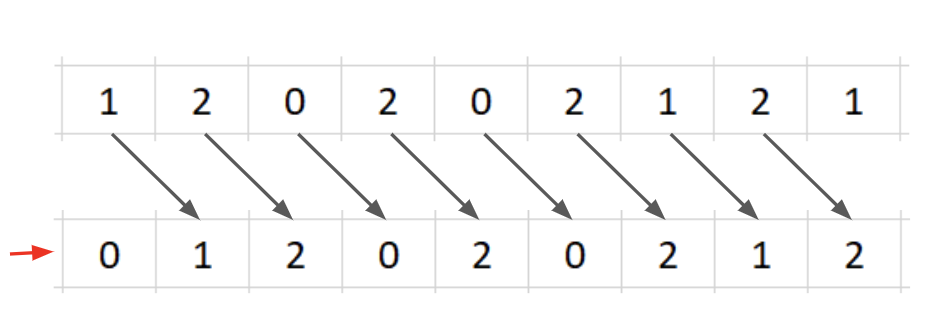
\includegraphics[width=0.45\textwidth]{images/arrayShift}
\begin{center}
	\textbf{Fig. 7} Example of shifting an array. \\
\end{center}

The shifting of arrays to move cars state to state is the bulk of the simulation and the problem we could boil down to what needed to be done in parallel. Before any parallel was integrated into our solution, we created a smaller subset problems to replicate one step in our simulation and use as a proof of concept.  \\

\hspace*{.2cm} Before being able to create and test the shifting of arrays in parallel, we had to fix one major issue that occurs during the parallelization of this type of problem, which was a loop carried dependency. The shifting of arrays depends on the ability of one state to look ahead or behind one iteration to move to the next spot.In other words, the current loop iteration looks ahead or behind one iteration to make the update. In a parallel design of array shifting, the process of shifting each position in the array would be divided among $p$ processes, which results in the following problem:

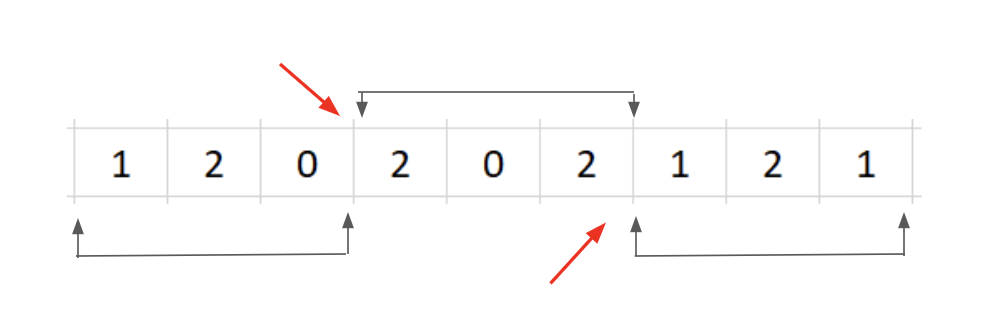
\includegraphics[width=0.45\textwidth]{images/dependency}
\begin{center}
	\textbf{Fig. 8} Loop carried dependency \\
\end{center}

Suppose there is an array of size 9 split up among 3 processes as seen in Fig. 7. The red arrows point out the spots where the dependency occurs, because each process needs data that another process is handling to complete its job correctly. The shifitng of arrays within a loop carries this dependency because a statement in one iteration of the loop depends on a statement in a different iteration of the loop. This means that the parallelization of shifting an array cannot be done simply by giving each process a size of the array to perform the shift on.  \\

\hspace*{.2cm} To solve this loop dependency issue we made use of next state arrays. The next state array is simply an array that holds the same value of the array to be shifted so that each process has access to the data it needs without it being changed anywhere else. The concept of a next state array successfully solves the loop dependency issue, but also adds extra overhead in continuously updating and storing such arrays for every state in the simulation, which will be touched on later. \\

\hspace*{.2cm} After solving this issue we ran subproblems of our simulation by testing the shifting of an array of size $20,000,000$ using a varying number of threads in OpenMP vs. Shifting sequentially. The timing results of these tests are shown in Fig. 8. \\

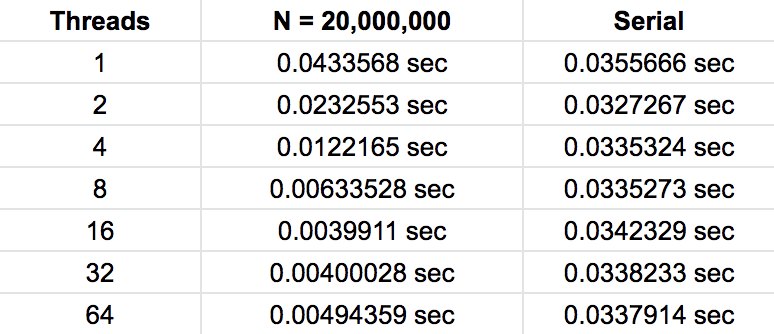
\includegraphics[width=0.45\textwidth]{images/subtest}
\begin{center}
	\textbf{Fig. 9} Parallel vs Sequential array shift \\
\end{center}

The number of threads performing the shift we varied from 1 to 64. The results show that a performance benefit started to occur immediately with the addition of a second thread. As the number of threads increased the performance also steadily grew compared to the results of the sequential shift. With these results we were able to confirm the parallelization technique we would be using and begin integrating into our actual simulation. \\
\hspace*{.2cm} Due to the logic heavy nature of the sequential solution, we had to decide on the most beneficial areas to parallel while keeping the integrity of the simulation. During any green light state in the simulation, the most work being done is happening on the outside, with cars driving away from the intersection or up to the intersection, while the cars in the green light lane are moving forward. The updating of all other cars requires the most work throughout each simulation state. This made us decide to parallelize all movement of cars happening outside of those moving because of the green light. By doing this, we make it so movement of cars in each lane is occurring in parallel, which is true for real traffic flow. So as cars move through the green light lanes, cars moving away and out of each road are being updated in parallel. To parallelize this aspect of the solution we parallelized the for loops responsible for updating each of the necessary areas of the road. OpenMP makes this process very simple to do, and because our project was extremely loop heavy, it makes it all the more viable of a tool.

\hspace*{.2cm} After integrating our parallel solution into our sequential project, we tested our simulation with a varying number of threads and problem sizes using stampede, similar to our subproblem tests. We used input sizes ranging from $20$ to $200,000$ and varied the number of threads from 1 to 64. The results we got back are shown in Fig. 9. \\ \\

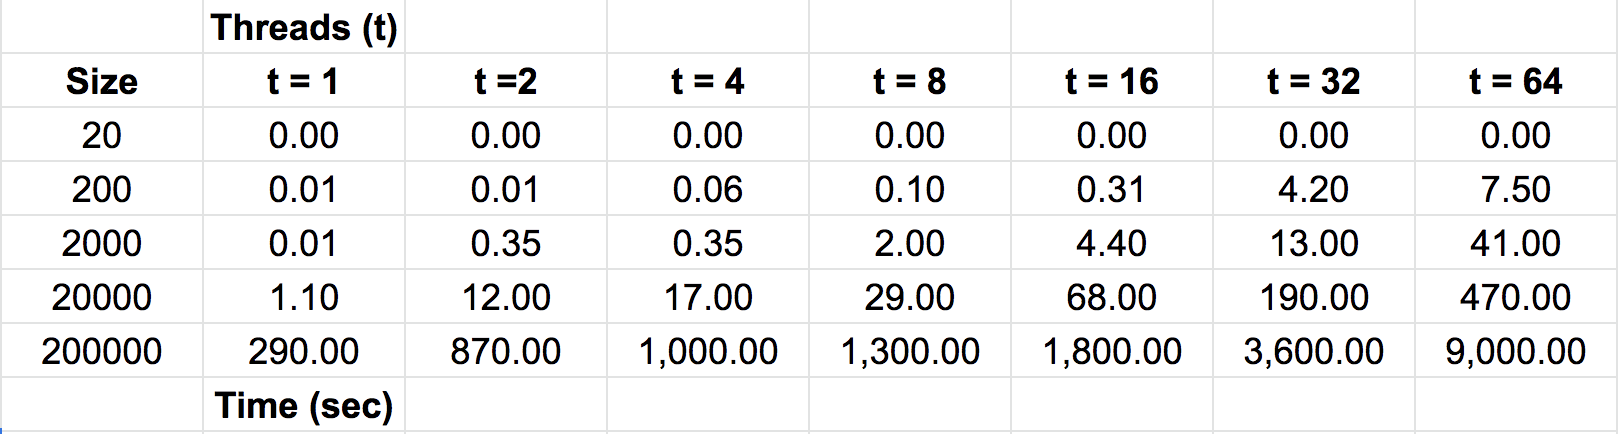
\includegraphics[width=0.45\textwidth]{images/results} \\
\begin{center}
	\textbf{Fig. 10} Parallel Simulation vs Sequential \\
\end{center}


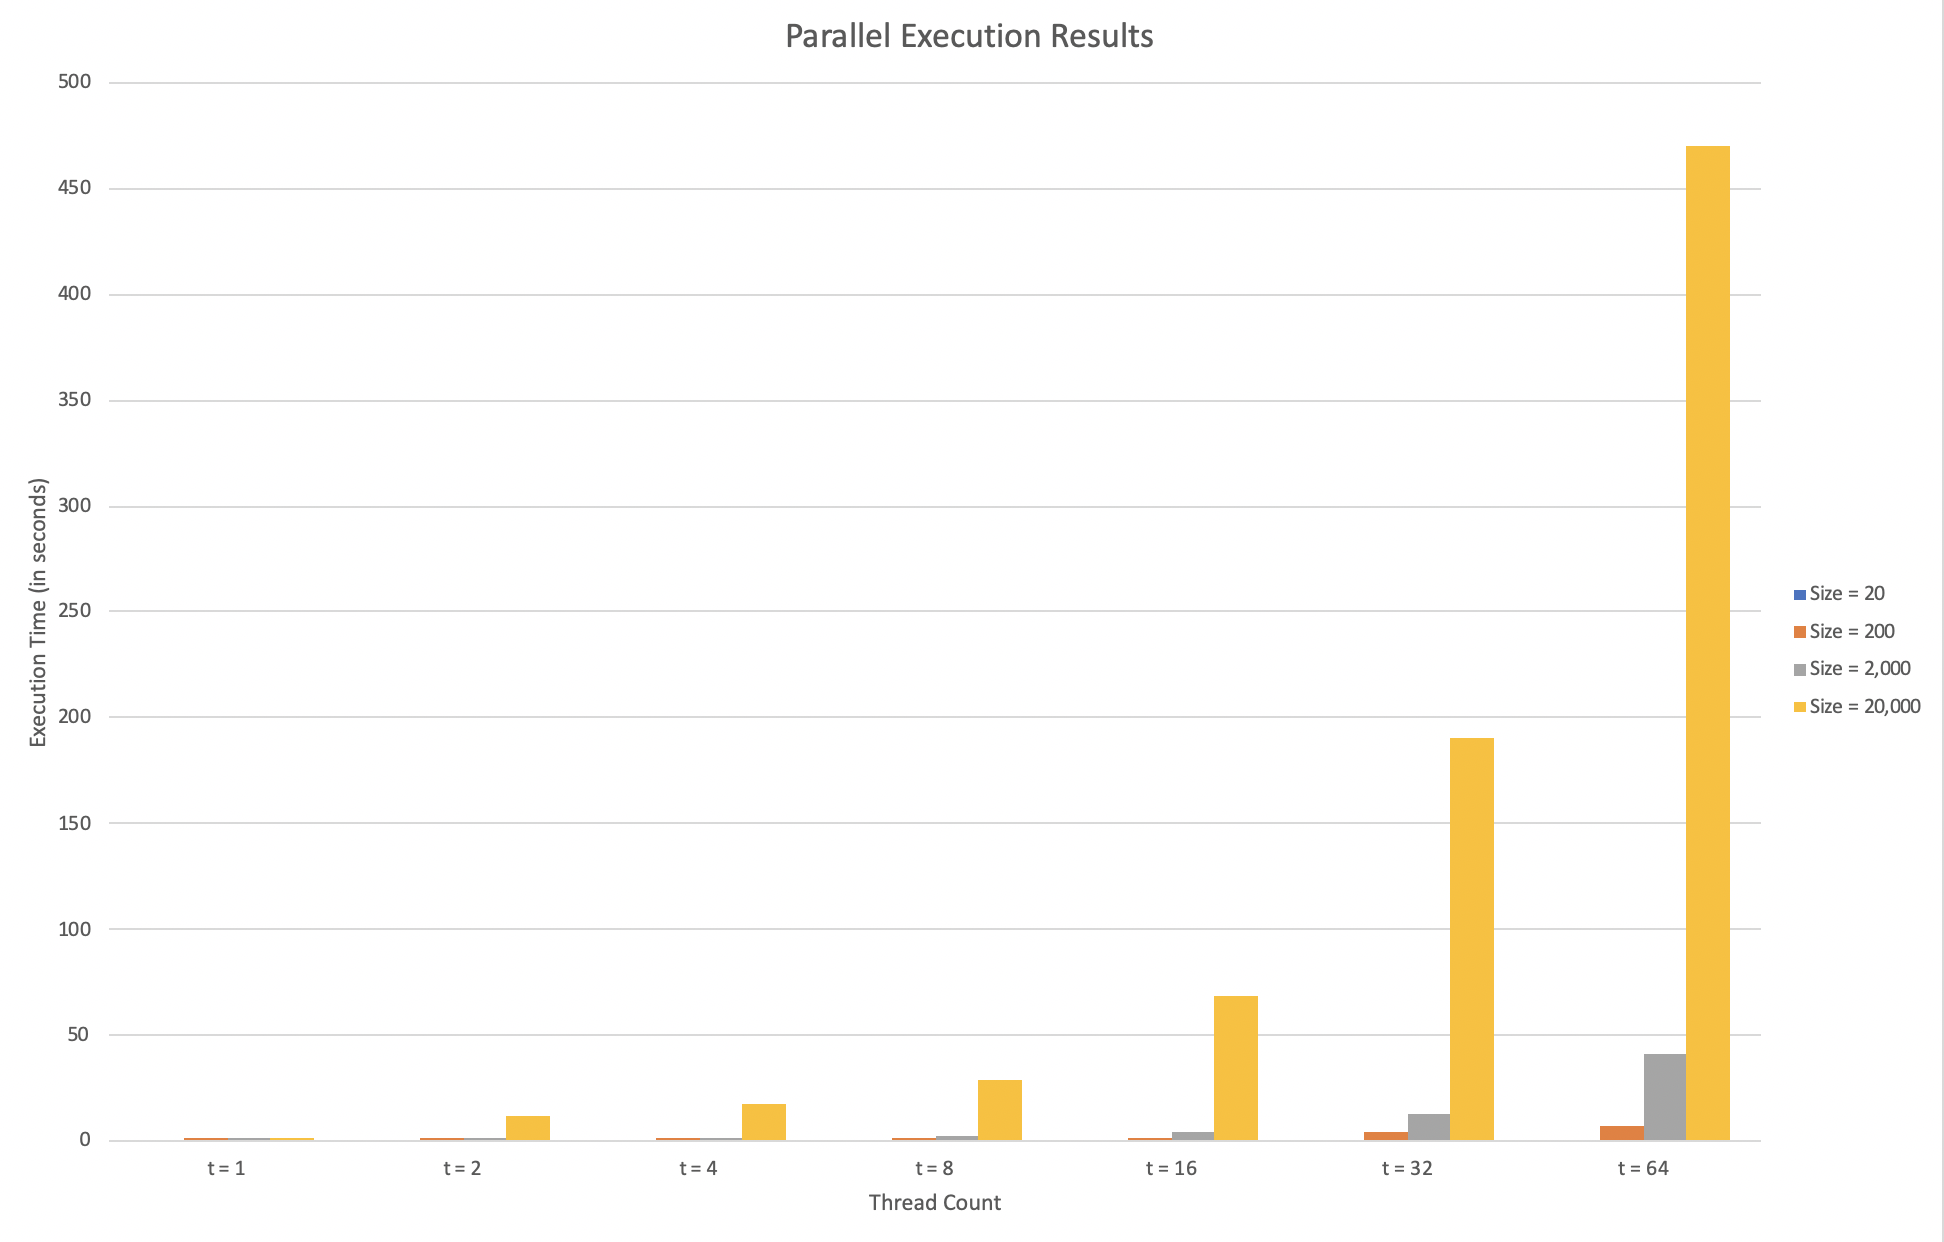
\includegraphics[width=0.45\textwidth]{images/timeVSthreads}
\begin{center}
	\textbf{Fig. 11} Parallel Execution Timing Results \\
\end{center}

\section{Summary of Results}
We observed that there were no performance benefits from using OpenMP based parallelization but rather our execution times got worse as we increased the number of threads. \\

\hspace*{.2cm}But going in a little deeper and understanding the timings tells us there is more to the story. The parts of the program that were parallelized were the shifting array state shifts in the automata that transitioned the cars to their next state in one direction. To make these shifts, we go through numerous other calculations involving various primitive data types and conditional statements. So, even though the actual part of shifting arrays is parallelized it doesn't reflect on the timings as compared to the calculations, since the shift is a smaller part of the program. \\

\hspace*{.2cm}The traffic simulation parallel project does the shift array differently from the serial program as it involves storing the elements of the array in a next state array in order to counter the loop carried dependencies. This is also an overhead in our parallelizing process, as duplicating the arrays for each state in the automata make the simulation slower. The parallelized version also has distinct OpenMP pragma calls for each of the lanes as the indexing inside the 'for' loops is handled differently. Hence, the parallel project pragma call couldn't be unified together. This results in a greater overhead of system calls for creation, separation, and termination of these threads. \\

\hspace*{.2cm}The project also faces the problem of accessing the critical section for each state simulation, hence making it difficult to parallelize the movement of cars in each of the North, South, East and West lanes. All these lanes need to access the intersection, and the critical section for their state simulations. Hence the lane shifts if parallelized in the previous stated manner would have to wait to check and see if all other lanes have left the intersection before it access it for each discrete state. This is because each state uses the critical section for all other states in the system, even when parallelized by lanes, this almost results in an inherently sequential simulation. \\

\hspace*{.2cm}Where this analysis does gets interesting, is by observing the percent change of execution time from the previous input size, per the number of threads: \\

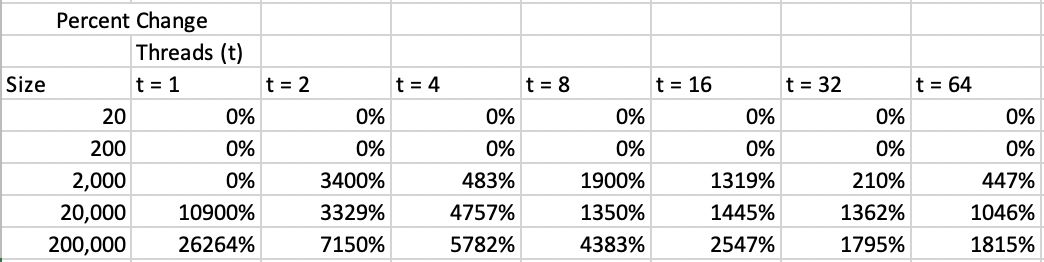
\includegraphics[width=0.45\textwidth]{images/percentChange}
\begin{center}
	\textbf{Fig. 12} Percent Change of Timing Results \\
\end{center}

As the thread count increases, and the input size increases, the percent change of execution time noticeably decreases.  With enough input, we predict that this will result in an eventual speed up, if the input size is large enough. As shown in the graph below, this trend can be observed: \\ \\
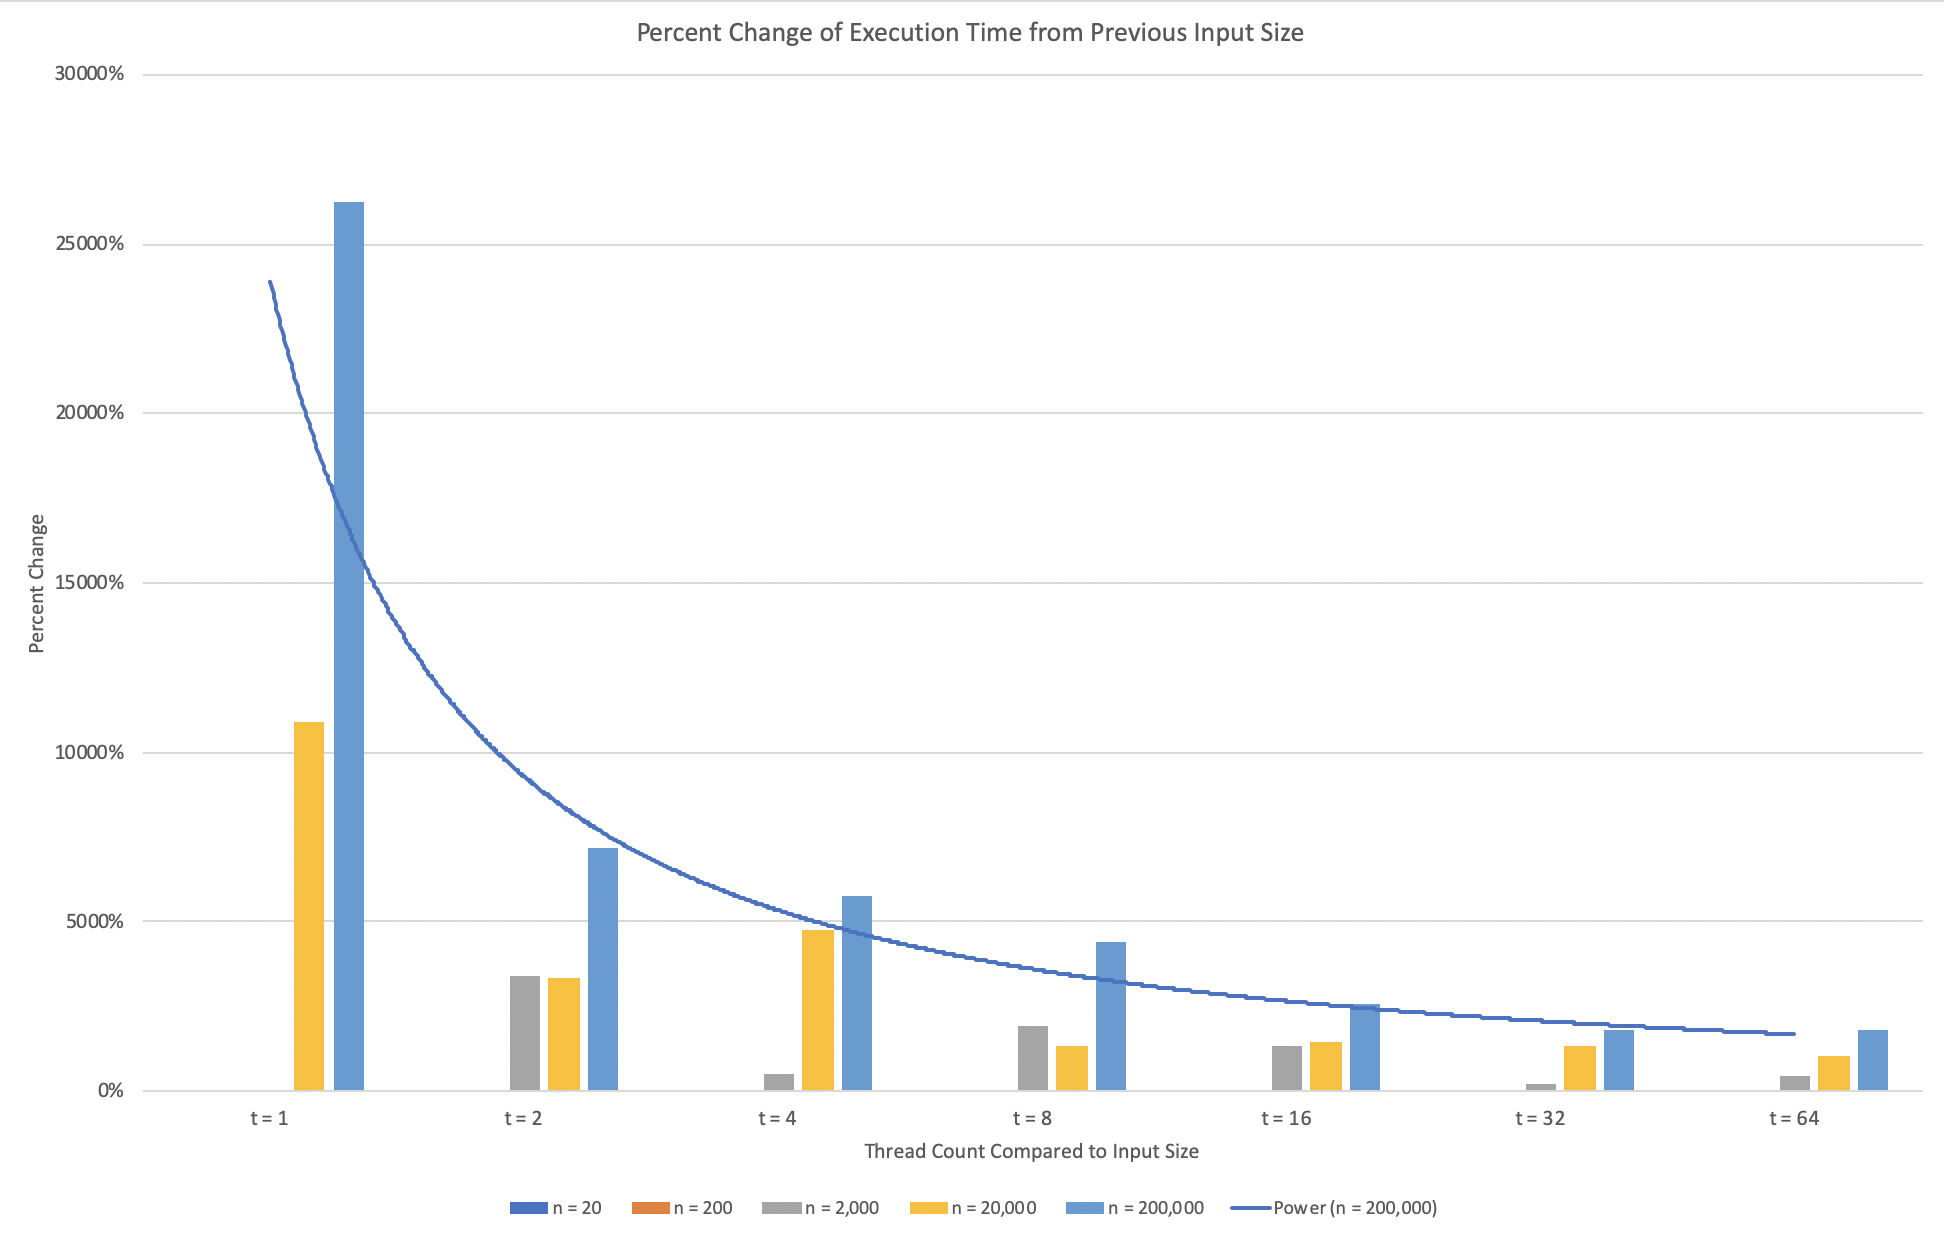
\includegraphics[width=0.45\textwidth]{images/percentChangeGraph}
\begin{center}
	\textbf{Fig. 12} Percent Change of Timing Results Graph \\
\end{center}

The graph divides the rate of change of execution time for the input sizes into the various thread count levels. As the number of threads increases, and the input size increases, you can see the expected result of more sustainable scalability, and the potential for possible speed up. \\

\section{Conclusions, Lessons Learned, and Future Work}
To summarize, this project was an attempt on parallelizing the discrete state transitions in a cellular automaton-based traffic simulation. Traditional parallelization attempt to decompose the system and predict next states, where this simulation keeps the system unified. \\

Our results show that the execution of the model with an increasing number of threads and input size results in a monumental increase in execution time. This was due to our limited computational power and time. To gain further insight, we would like to continue running this simulation for input sizes of 2,000,000 all the way to 2,000,000,000 to see how execution time scales.  When we ran state simulation change tests, we found that the shift array operation that we parallelized had noticeable performance increases after an input size 20,000,000 as the number of threads was increased. We predict a similar critical point for our simulation. Where our project did succeed was starting to see a decrease in the relative percent change of execution time as the input size was increased. Sequential scaled very poorly, and as more threads were added, the scalability was improved. \\

In the future, simulations should be run and repeated with large variations from small to massive input sizes. Our results and analysis were limited by the time and computational power available to us. More executions of the same size would provide more solidified and accurate execution timing results. Another analysis we would have liked to include would be comparing the timing of a similar input and simulation to a program that uses a decomposition technique to see how the execution times and scalability would differ.
 \\

For future work, in terms of simulation logic, we would like to implement more unpredictable factors in the model such as acceleration, lane changes, relative light timings based on the car counts in each lane, etc.  This would make the automaton less stable, and would be interesting to see how it would be able to scale with our approach, or if a decomposed system is truly the best technique for a parallelized traffic simulation.
\\


\bibliographystyle{ieeetr}
\bibliography{HPC_Project}

\end{document}